\documentclass[preprint, 10pt]{sigplanconf}

\usepackage{uri}
\usepackage{amsmath}
\usepackage{mathtools}
\usepackage{amsthm}
\usepackage{amssymb}
\usepackage{semantic}
\usepackage{graphicx}
\usepackage{cases}
\usepackage{xcolor}
\usepackage{xspace}
\usepackage{hyperref}
\usepackage{stmaryrd}
\usepackage[all]{xy}

\newcommand{\eg}{\textit{e.g.}\xspace}
\newcommand{\ie}{\textit{i.e.}\xspace}
\newcommand{\TODO}[1]{\textbf{\textcolor{red}{[ TODO: #1]}}}

\newcommand{\ignore}[1]{}


%%% from this paper
\newcommand{\con}[1]{\ensuremath{\mathsf{consistent}(#1)}}
\newcommand{\seqcon}[1]{\ensuremath{\mathsf{seq\_con}(#1)}}
\newcommand{\mread}[2]{\ensuremath{\mathsf{read}(#1, #2)}}
\newcommand{\mwrite}[2]{\ensuremath{\mathsf{write}(#1, #2)}}
\newcommand{\malloc}[2]{\ensuremath{\mathsf{alloc}(#1, #2)}}
\newcommand{\mfree}[1]{\ensuremath{\mathsf{free}(#1)}}
%\newcommand{\cccando}[2]{\ensuremath{\mathsf{can\_do_{CC}}(#1, #2)}}
\newcommand{\hb}[0]{<_{\mathrm{hb}}}
\newcommand{\po}[0]{<_{\mathrm{po}}}
\newcommand{\sw}[0]{<_{\mathrm{sw}}}
\newcommand{\word}[0]{<_{\mathrm{w}}}

%%% from Radish paper
\newcommand{\Dom}{{\sf Dom}}
\newcommand{\Trace}{\alpha}
\newcommand{\Tid}{t}
\newcommand{\TidU}{u}
\newcommand{\Address}{x}
\newcommand{\AddressY}{y}
\newcommand{\Value}{b}
\newcommand{\Lock}{m}
\newcommand{\Op}[1]{o_{#1}}
% \newcommand{\ReadOp}[1]{read #1}
% \newcommand{\WriteOp}[3]{wr_{#1}(#2)}
% \newcommand{\AcqOp}[2]{acq_{#1}(#2)}
% \newcommand{\RelOp}[2]{rel_{#1}(#2)}
\newcommand{\Clock}{c}
%\newcommand{\Epoch}[2]{(#1, #2)}
\newcommand{\VC}{V}
\newcommand{\VCFont}{}
\newcommand{\ThreadVC}[1]{\VCFont{C}_{#1}}
\newcommand{\LockVC}[1]{\VCFont{L}_{#1}}
\newcommand{\ReadVC}[1]{\VCFont{R}_{#1}}
\newcommand{\WriteVC}[1]{\VCFont{W}_{#1}}
\newcommand{\VCInc}[2]{inc_{#1}(#2)}
\newcommand{\SuchThat}{\ \text{s.t.}\ }
\newcommand{\Bind}{\ .\ }

\newcommand{\VCalg}{\textsc{VectorClock}\xspace}
%% from SlimFast paper
\newcommand{\FT}{\textsc{FastTrack}\xspace}
\newcommand{\Constant}{O($1$)\xspace}
\newcommand{\Linear}{O($n$)\xspace}
\newcommand{\Epoch}{\textit{Epoch}\xspace}
\newcommand{\VectorClock}{\textit{Vector Clock}\xspace}
\newcommand{\Rule}[1]{\textsc{#1}}
\newcommand{\VCMax}{\sqcup}
\newcommand{\VCCompare}{\sqsubseteq} 
\newcommand{\EpochCompare}{\preceq}
\newcommand{\EmptyEpoch}{\bot_e}
%\newcommand{\EmptyVC}{\bot_V} % TODO: not used

%%% Semantics
\newcommand{\meanl}{\ensuremath{[ \! [}}
\newcommand{\meanr}{\ensuremath{] \! ]}}
\newcommand{\means}[1]{\ensuremath{\meanl #1 \meanr}}


%%% our language's concrete syntax
\newcommand{\assign}[2]{#1\ \texttt{:=}\ #2}
\newcommand{\load}[2]{#1\ \texttt{:= load}\ #2}
\newcommand{\store}[2]{\texttt{store}\ #2\ #1}
\newcommand{\lock}[1]{\texttt{lock}\ #1}
\newcommand{\unlock}[1]{\texttt{unlock}\ #1}
\newcommand{\spawn}[2]{\texttt{spawn}\ #1\ #2}
\newcommand{\wait}[1]{\texttt{wait}\ #1}
\newcommand{\assert}[2]{\texttt{assert(}#1\ \texttt{<=}\ #2\texttt{)}}
\newcommand{\move}[2]{\ensuremath{\mathsf{move}(#1, #2)}}
\newcommand{\setvc}[2]{\ensuremath{\mathsf{set}(#1, #2)}}
\newcommand{\incvc}[2]{\ensuremath{\mathsf{inc}(#1, #2)}}
\newcommand{\maxa}[2]{\ensuremath{\mathsf{max}(#1, #2)}}
\newcommand{\maxvc}[2]{\ensuremath{\mathsf{merge}(#1, #2)}}
\newcommand{\lea}[2]{\ensuremath{\mathsf{lea}(#1, #2)}}
\newcommand{\vcle}[2]{\ensuremath{\mathsf{hb\_check}(#1, #2)}}
%\newcommand{\instr}[2]{\ensuremath{\mathsf{instrument}(#1, #2)}}
\newcommand{\instr}[2]{\ensuremath{\means{#2}_{#1}}}
\newcommand{\instrp}[1]{\ensuremath{\mathsf{instrument}(#1)}}
\newcommand{\cfg}[2]{\ensuremath{(#1, #2)}}
\newcommand{\anarrow}[2]{\ensuremath{\xrightarrow{#2}_{#1}}}
\newcommand{\exec}[5]{\ensuremath{\cfg{#1}{#2} \anarrow{#3}{#4} #5}}
\newcommand{\execstar}[4]{\ensuremath{\cfg{#1}{#2} \tto{#3} #4}}
\newcommand{\iexec}[4]{\ensuremath{\cfg{#1}{#2} \Rightarrow_{#3} #4}}
\newcommand{\execstart}[4]{\ensuremath{\cfg{#1}{#2} \rightarrow^{*}_{#3} #4}}
\newcommand{\execstarm}[4]{\ensuremath{\cfg{#1}{#2} \rightarrow^{*}_{\neg #3} #4}}
\newcommand{\execs}[3]{\ensuremath{ \xrightarrow{#2}_{#1} #3}}
\newcommand{\execstars}[2]{\ensuremath{ \tto{#1} #2}}
\newcommand{\iexecs}[2]{\ensuremath{ \Rightarrow_{#1} #2}}
\newcommand{\execstarts}[2]{\ensuremath{ \rightarrow^{*}_{#1} #2}}
\newcommand{\execstarms}[2]{\ensuremath{ \rightarrow^{*}_{\neg #1} #2}}
\newcommand{\iexecstar}[3]{\ensuremath{(#1, #2) \Rightarrow^{*} #3}}



%from StackExchange, a better xrightarrow^*
\newcommand{\tto}[1]{\mathrel{
  \vphantom{\xrightarrow{#1}}
  \smash{\xrightarrow{#1}}
  \vphantom{\to}^{*}}
}
\newcommand{\tTo}[1]{\mathrel{
  \vphantom{\xrightarrow{#1}}
  \smash{\xRightarrow{#1}}
  \vphantom{\to}^{*}}
}

\hyphenation{Comp-Cert}

\newtheorem{lemma}{Lemma}
\newtheorem{theorem}{Theorem}
\newtheorem{definition}{Definition}
\newtheorem{principle}{Principle}


\begin{document}

\special{papersize=8.5in,11in}
\setlength{\pdfpageheight}{\paperheight}
\setlength{\pdfpagewidth}{\paperwidth}

%\conferenceinfo{PLDI '16}{June 13--17, 2016, Santa Barbara, California, United States} 
%\copyrightyear{2016}
%\copyrightdata{978-1-nnnn-nnnn-n/yy/mm} 
%\doi{nnnnnnn.nnnnnnn}

% Uncomment one of the following two, if you are not going for the 
% traditional copyright transfer agreement.

%\exclusivelicense                % ACM gets exclusive license to publish, 
                                  % you retain copyright

%\permissiontopublish             % ACM gets nonexclusive license to publish
                                  % (paid open-access papers, 
                                  % short abstracts)

\titlebanner{}        % These are ignored unless
\preprintfooter{}   % 'preprint' option specified.

\title{Verifying Dynamic Race Detection}
\ignore{\authorinfo{William Mansky \and Yuanfeng Peng \and Steve Zdancewic \and Joseph Devietti}
           {University of Pennsylvania}
           {wmansky@seas.upenn.edu, yuanfeng@cis.upenn.edu, stevez@cis.upenn.edu, devietti@cis.upenn.edu}}
\authorinfo{}{}{}
\maketitle

\begin{abstract}
Writing race-free concurrent code is notoriously difficult, and races can result in bugs that are difficult to isolate and reproduce. Dynamic race detection is often used to catch races that cannot (easily) be detected statically. One approach to dynamic race detection is to instrument the potentially racy code with operations that store and compare metadata, where the metadata implements some known race detection algorithm (e.g. vector-clock race detection). In this paper, we describe the process of formally verifying several algorithms for dynamic race detection. We then lay out an instrumentation pass for race detection in a simple language, and present a mechanized formal proof of its correctness: all races in a program will be caught by the instrumentation, and all races detected by the instrumentation are possible in the original program.\ignore{ During the verification process, we discovered issues \TODO{tone this down?} in both the paper proof and the implementation of the \FT race detection algorithm.}
\end{abstract}

%\category{CR-number}{subcategory}{third-level}

%\keywords
%dynamic race detection, interactive theorem proving

\section{Introduction}

Multicore processors have steadily invaded a broad swathe of the computing ecosystem in everything from datacenters to smart watches. Writing multithreaded code for such platforms can bring good performance but also a host of programmability challenges. One of the key challenges is dealing with data races, as the presence of a data race introduces non-sequentially-consistent~\cite{manson_java_2005} and in some cases undefined~\cite{boehm_foundations_2008} behavior into programs, making program semantics very difficult to understand. Races are not detected by default in current language runtimes, though there are many systems that provide sound and complete data race detection via dynamic analysis~\cite{djit+,fasttrack,slimstate} to help programmers detect and remove data races from their programs. 

While these analyses have been proven correct, such proofs have two main shortcomings: they are proofs of the algorithms, instead of the implementations, and they are paper proofs instead of machine-checked proofs. Because of these shortcomings, it is possible that a race detector does not faithfully implement its algorithm, or that the algorithm itself is not fully correct. Moreover, it still remains to be shown that the implementation, often done via code instrumentation, does not itself introduce or mask races, and that, in the absence of races, the program's behavior is unchanged.

In this paper, we seek to rectify these concerns and place dynamic race detection on a provably correct foundation for the first time\footnote{All proofs are fully machine-checked in Coq. We have submitted them as non-anonymous supplementary material, and intend to submit a documented version for artifact evaluation.}. We begin by formalizing the proof of the classic vector-clock race detection algorithm~\cite{vcfidge,vcmattern} using the Coq interactive theorem prover~\cite{coq}. Having established the correctness of this base algorithm, we extend our work along two dimensions. 

\begin{figure}[t]
\centering
 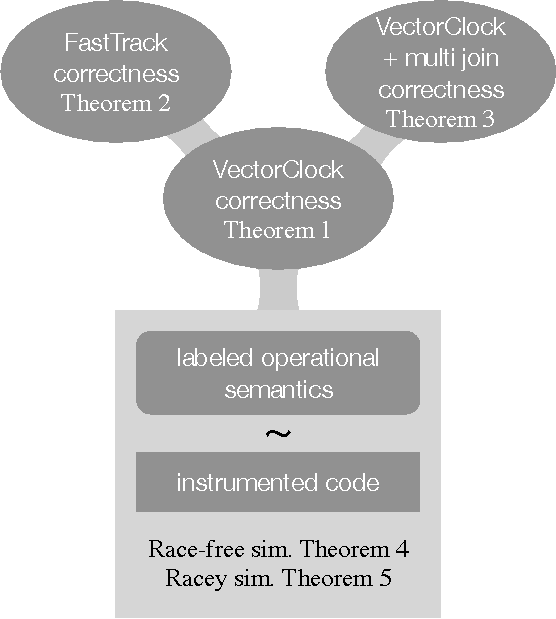
\includegraphics[width=0.6\columnwidth]{overview.pdf}
 \caption{An overview of our work, showing verified algorithms (top) and our approach to verified instrumentation code via a labeled operational semantics.}
 \label{f:overview}
\end{figure}

We first explore the \textbf{algorithmic dimension} (ellipses in \autoref{f:overview}), by formally establishing the correctness of the \FT algorithm~\cite{fasttrack}. \FT includes several significant optimizations over the base vector-clock algorithm. We find that the correctness of \FT can be demonstrated by proving its equivalence to the vector-clock algorithm, which is a more straightforward process than demonstrating correctness in isolation, and likely lends itself to formalizing additional algorithms with reduced effort. \ignore{Our verification efforts have revealed a small issue in the paper proof that, while fixable, illustrates the potential dangers that stem from best-effort proofs. We have repaired this issue in our proof of \FT, establishing that the algorithm is correct.} We also verify an extension of the base vector-clock algorithm that allows multiple joins of the same thread, as modern threading packages do.

We next explore the \textbf{implementation dimension} (rectangles in \autoref{f:overview}), by formally establishing in Coq the correctness of an implementation of vector-clock race detection on a simple imperative language with threads. Given a program written in our language, our race detector adds instrumentation, written in the same language, to perform vector-clock race detection on the program. We demonstrate that this instrumentation correctly implements the vector-clock algorithm, again leveraging our previous verification effort. We also prove that our implementation preserves the program's semantics in the absence of races. This verification is much more difficult than proving the correctness of the algorithms, since it must deal directly with the details of the implementation language and the concurrency model; we must precisely define the relation between uninstrumented and instrumented memory states, and prove noninterference of the code added by the instrumentation. \ignore{While constructing our implementation, we consulted the existing implementation of \FT for guidance, and our verification process brought to light an example of extraneous work performed by the current \FT implementation. This issue is unlikely to have come to light otherwise, but when proving our implementation equivalent to the abstract algorithm such discrepancies were quickly revealed. This again demonstrates the value of formal verification over best-effort implementation, ensuring that an implementation does no less, and no more, than is necessary for correctness.}

To the best of our knowledge, ours is the first work to adopt formal verification for either race detection algorithms \emph{or} their implementations. Moreover, we believe our general approach may be useful as a template for verifying a broad range of dynamic analyses, especially in the challenging domain of analyses for parallel programs. Verification is critical to help ensure that debugging tools are themselves free from bugs.

This paper makes the following contributions:
\begin{itemize}
\item We present a method for verifying a dynamic data race detector from the algorithmic level through to its implementation.
\item We give the first machine-checked proofs of correctness of the vector-clock and \FT data race detection algorithms.
\item We give the first verified implementation of vector-clock race detection on a simple, imperative multithreaded language.
\ignore{\item We uncover issues in the paper proof of correctness for \FT and in its current implementation that are unlikely to have been revealed without our verification efforts. We repair these issues in our own proofs and implementation.}
\end{itemize}
Along the way, we discovered that one lemma in the paper proof of \FT needed strengthening, and noticed a discrepancy between the \FT algorithm and one version of its implementation (which was corrected in a later version based on our feedback to the \FT authors). This highlights the value of formal verification for obtaining correct algorithms and implementations.

The remainder of this paper is organized as follows. In Section~\ref{strategy}, we lay out our approach to verifying dynamic race detection algorithms and their implementations. In Section~\ref{algorithms}, we state and verify several algorithms for race detection. In Sections~\ref{language} and \ref{verification}, we describe an instrumentation pass that implements dynamic race detection, and explain the verification process in detail. We compare our approach to related work in Section~\ref{related}, and evaluate our results and describe future work in Section~\ref{conclusion}.

\section{Proof Strategy}
\label{strategy}
Our goal for each algorithm and program transformation presented in this paper is to prove that it implements sound and complete race detection, i.e., that it raises an alarm in all racy executions and only racy executions. However, as much as possible, we prefer not to do this by referring back to the base definition of racy executions. We begin by stating and proving correctness of a simple vector-clock race detection algorithm, by direct relation to the definition of a race. We then prove further results---the correctness of a more sophisticated algorithm, and of an instrumentation pass meant to implement the simple algorithm---by relating them to the verified base algorithm. We may think of this hierarchy in terms of specifications and refinement: we begin by proving that the base algorithm refines the abstract specification of race detection, and then use it in turn as a specification refined by more complex or detailed mechanisms. This allows us to separate concerns and avoid duplicating proof effort, but it also serves as further validation of the base vector-clock algorithm: by showing that it is \emph{two-sided}, that is, that it both implements a higher-level specification of its desired behavior and is implemented by more concrete systems, we gain confidence that it is correctly stated (and not, e.g., vacuously correct).

Our approach to verifying instrumentation has three major steps. First, we describe our race detection algorithm abstractly, separately from the details of any programming language. We verify this algorithm against a high-level specification of the property we want to guarantee (in this case, soundness and completeness). Secondly, we define the semantics of a target language, labeled with the abstract operations produced by each step. This means that from each execution of an uninstrumented program, we can use the algorithm to determine the behavior we \emph{would have observed} if the program was correctly instrumented. Thirdly, we define our instrumentation pass, and also write a bigger-step semantics for instrumented programs in which an instruction executes together with its instrumentation in a single step. This strategy is analogous to that used in other proof efforts~\cite{softbound}, and makes it easier to directly relate executions of an instrumented program to executions of the original program. Given the bigger-step semantics, the proof of correctness of the instrumentation then breaks down into two parts: a proof of simulation between the bigger-step semantics and ``would have observed'' semantics of the uninstrumented program, and a proof that the bigger-step semantics completely captures the possible behaviors of any instrumented program. This three-step approach has applications beyond race detection: we believe that it could be applied to simplify the verification of any kind of instrumentation for dynamic checks, including memory safety and atomicity violation checking. The approach is particularly useful when verifying instrumentation of concurrent programs, since we are able to isolate all reasoning about interference between threads in the latter half of the third step---characterizing the possible behaviors of the instrumented program---and otherwise reason more or less sequentially.

\section{Race Detection Algorithms}
\label{algorithms}
We begin by reviewing the classic vector-clock race detection algorithm~\cite{vcmattern, vcfidge}, which we call \VCalg, and briefly describing its verification in Coq. We then turn to the \FT~\cite{fasttrack} algorithm and its verification both by simulation with \VCalg and by direct proof, followed by the verification of a variant of \VCalg that handles multiple joins to the same thread.

% NB: VC stuff borrowed from Joe's Radish paper [ISCA '12]

\subsection{Defining Data Races}
Data races are formally defined in terms of a \emph{happens-before} relation $\hb$, a partial order over events in a program trace~\cite{lamporthb}. Events consist of $\mathit{rd}(t, x)$ and $\mathit{wr}(t, x)$ where a thread $t$ reads or writes a memory location $x$, lock operations $\mathit{acq}(t, m)$ and $\mathit{rel}(t, m)$ where a thread $t$ acquires or releases a lock $m$, $\mathit{fork}(t, u)$ where a thread $t$ creates a new thread $u$, and $\mathit{join}(t, u)$ where a thread $t$ joins with a thread $u$. Given events $a$ and $b$, we say $a$ \emph{happens before} $b$ (and $b$ \emph{happens after} $a$), written $a \hb b$, if: (1) $a$ precedes $b$ in program order in the same thread; or (2) $a$ precedes $b$ in synchronization order $\sw$, \eg, if $a$ is thread $\Tid$ releasing a lock $\Lock$, and $b$ is thread $\TidU$ subsequently acquiring it; or (3) $(a,b)$ is in the transitive closure of program order and synchronization order.
% Synchronization order also induces happens-before ordering on other synchronization events such as thread fork to thread start and thread termination to thread join.
Two events not ordered by happens-before are \emph{concurrent}.  Two memory accesses to the same address form a \emph{data race} if they are concurrent and at least one is a write.

\subsection{Vector-Clock Race Detection}
\label{vector-clocks}


\newcommand{\bigcell}[2][c]{% hat tip to http://tex.stackexchange.com/a/19678
  \begin{tabular}[#1]{@{}c@{}}#2\end{tabular}}

\begin{figure*}[t]
\footnotesize
\centering
\begin{tabular}{cp{1cm}c}

\bigcell{
\inference[\Rule{Acquire}]{C' = C[t := (C_t \VCMax L_m)]}{(C, L, R, W) \xRightarrow{\mathit{acq}(t, m)} (C, L, R, W)}\\\\

\inference[\Rule{\Rule{Release}}]{L' = L[m := C_t] \\ C' = C[t := \mathit{inc}_t(C_t)]}{(C, L, R, W) \xRightarrow{\mathit{rel}(t, m)} (C', L', R, W)} \\\\

\inference[\Rule{\Rule{Fork}}]{C' = C[u := C_u \VCMax C_t, t := \mathit{inc}_t(C_t)]}{(C, L, R, W) \xRightarrow{\mathit{fork}(t, u)} (C', L, R, W)}\\\\

\inference[\Rule{Join}]{C' = C[t := C_t \VCMax C_u, u := \mathit{inc}_u(C_u)]}{(C, L, R, W) \xRightarrow{\mathit{join}(t, u)} (C', L, R, W)}

} & &

\bigcell{
\inference[\Rule{\Rule{Read}}]{W_x \VCCompare C_t \\ R' = R[x := R_x[t := C_t(t)]] }{(C, L, R, W) \xRightarrow{\mathit{rd}(t, x)} (C, L, R', W)}\\\\

\inference[\Rule{ReadNoChange}]{R_x = C_t(t)}{(C, L, R, W) \xRightarrow{\mathit{rd}(t, x)} (C, L, R, W)}\\\\

\inference[\Rule{\Rule{Write}}]{R_x \VCCompare C_t \qquad W_x \VCCompare C_t \\ W' = W[x := R_x[t := C_t(t)]] }{ (C, L, R, W) \xRightarrow{\mathit{wr}(t, x)} (C, L, R, W') }\\\\

\inference[\Rule{WriteNoChange}]{W_x = C_t(t)}{(C, L, R, W) \xRightarrow{\mathit{wr}(t, x)} (C, L, R, W)}
}
\end{tabular}
\caption{\VCalg operational semantics}
\label{f:semvc}
\end{figure*}

One common algorithm for dynamic race detection is to use \emph{vector clocks} to track the happens-before relation during
execution \cite{vcfidge,vcmattern}.  A vector clock $\VC$ stores one (nonnegative) integer
logical clock per thread; we write $\VC(\Tid)$ for the data associated with thread $\Tid$ in clock $\VC$.

  There are three key operations on vector clocks.
\emph{Union} is the element-wise maximum of two vector clocks:
$\VC_1 \VCMax \VC_2 = \VC_3 \SuchThat \forall \Tid.\ \VC_3(\Tid) =
\max(\VC_1(\Tid), \VC_2(\Tid))$. \emph{Comparison} is the element-wise
comparison of two vector clocks: $\VC_a \VCCompare \VC_b$ is defined to mean $\forall
\Tid.\ \VC_a(\Tid) \leq \VC_b(\Tid)$.  Finally, \emph{increment} increases a single component of a vector clock, defined as $\mathit{inc}_t(V) = \lambda u.\ \mathrm{~if~} u=t \mathrm{~then~} V(u)+1 \mathrm{~else~} V(u)$.

The state of a vector-clock race detector is a tuple $(C, L, R, W)$ of collections of vector clocks, where:
\begin{itemize}
%\setlength{\itemsep}{1pt}
%\setlength{\parskip}{0pt}
%\setlength{\parsep}{0pt}
%% \item For each thread $\Tid$, vector clock $\ThreadVC{\Tid}$ represents the last
%%   event in each thread that happens before $\Tid$'s current logical time.
%% \item For each lock $\Lock$, vector clock $\LockVC{\Lock}$ represents the last
%%   event in each thread that happens before the last release of $\Lock$.  
%% \item For each address $\Address$, vector clock $\WriteVC{\Address}$ represents
%%   the time of each thread's last write to $\Address$.
%% \item For each address $\Address$, vector clock $\ReadVC{\Address}$ represents
%%   the time of each thread's last read of $\Address$ \emph{since the last write
%%     by any thread}.  If thread $t$ has not read $\Address$ since this write,
%%   then $\ReadVC{\Address}(\Tid) = 0$.
\item
 Vector clock $\ThreadVC{\Tid}$ stores the last time in each thread that happens before thread $\Tid$'s current logical time.
\item
 Vector clock $\LockVC{\Lock}$ stores the last time in each thread that happens before the last release of lock $\Lock$.  
\item
 Vector clock $\ReadVC{\Address}$ stores
  the time of each thread's last read of address $\Address$.
\item
 Vector clock $\WriteVC{\Address}$ stores
  the time of each thread's last write to address $\Address$.
\end{itemize}

Initially, all $\LockVC{}$, $\ReadVC{}$, and $\WriteVC{}$ vector clocks are
set to $\bot_V$, where $\forall \Tid \Bind \bot_V(\Tid) = 0$.  Each thread $\Tid$'s
initial vector clock is $\ThreadVC{\Tid}$, where $\ThreadVC{\Tid}(\Tid) = 1$
and $\forall \TidU \neq \Tid \Bind \ThreadVC{\Tid}(\TidU) = 0$.  

\VCalg's operational semantics are presented in \autoref{f:semvc}. Each rule has the form $S \xRightarrow{a} S'$, meaning that when the current vector clock state is $S$ and the next event is $a$, the next vector clock state is $S'$. When a thread $\Tid$ acquires a lock $\Lock$ (the \Rule{Acquire} rule) we update $\ThreadVC{\Tid}$ to $\ThreadVC{\Tid} \VCMax \LockVC{\Lock}$.  By acquiring lock $\Lock$, thread $\Tid$ has synchronized with all events that happen before the last release of $\Lock$, so all these events happen before all subsequent events in $\Tid$.  When $\Tid$ releases a lock $\Lock$ (the \Rule{Release} rule), we update $\LockVC{\Lock}$ to $\ThreadVC{\Tid}$, capturing all events that happen before this release.  We then increment $\Tid$'s entry in its own vector clock $\ThreadVC{\Tid}$ to ensure that subsequent events in $\Tid$ do not appear to happen before the release $\Tid$ just performed.  The \Rule{Fork} and \Rule{Join} rules are similar to \Rule{Release} and \Rule{Acquire}, respectively. The increment $\mathit{inc}_u(C_u)$ in \Rule{Join} is needed to preserve the invariant that $\ThreadVC{\TidU}(u)$, thread $\TidU$'s entry for itself, is always higher than any other thread's entry for $\TidU$.

When $\Tid$ reads a location $\Address$ (the \Rule{Read} rule), we check if $\WriteVC{\Address} \VCCompare \ThreadVC{\Tid}$.  If this check fails, there is a previous write to $\Address$ that did not happen before this read, so there is a data race. (Note that the algorithm is considered to detect a race when it is \emph{stuck}, that is, when there is no rule that can be applied for the next operation; when a state $\sigma$ is stuck on an operation $o$, we write $\sigma \not\xRightarrow{o}$.) Otherwise, we set $\Tid$'s entry in $\ReadVC{\Address}$ to $\Tid$'s current logical clock, $\ThreadVC{\Tid}(\Tid)$.  It often arises that $\Tid$ will read the same location repeatedly without an intervening change in its own clock value $\ThreadVC{\Tid}(\Tid)$. The \Rule{ReadNoChange} rule covers this case, in which no metadata updates are necessary.

Writes operate similarly to reads, with an additional check in the \Rule{Write} rule that $\ReadVC{\Address} \VCCompare \ThreadVC{\Tid}$ to ensure that all previous reads of $\Address$ are well-ordered before the current write. This is not necessary in the \Rule{Read} case because two concurrent reads are not considered to race.

%\paragraph{Optimizations of Vector Clocks}
%Thus every read and write of $\Address$
%must happen after the last write to $\Address$ and every write to $\Address$
%must also happen after all last reads of $\Address$ since the last write to
%$\Address$.  

\subsubsection{Correctness}
Correctness for dynamic race detection is phrased in terms of \emph{soundness} and \emph{completeness}. Soundness means that if the algorithm runs to completion, then there was no race in the program trace; completeness means that given a trace without races, the algorithm does not get stuck.
\begin{theorem}\label{vc-correct}\VCalg is sound and complete.\end{theorem}
The soundness and completeness of \VCalg follows from the fact that the $\sqsubseteq$ relation between vector clocks precisely models the happens-before relation. Our Coq formalization follows the proof outline given in the presentation of \FT~\cite{fasttrack} (with the change described in Section~\ref{bug}), which can be straightforwardly translated into Coq. The main invariant of the algorithm is that $C_t(t) > C_u(t)$, that is, each thread always has a higher timestamp for itself than any other thread has for it. This guarantees that no operation by a thread $t$ can be seen by another thread $u$ (without detecting a race) until $t$ has synchronized with $u$.

\subsection{\FT}

% joe: lifted from the SlimFast paper

The \FT algorithm~\cite{fasttrack} leverages the observation that, by the definition of a data race, all writes to an address must be totally ordered in race-free traces. \FT accordingly adopts a more sophisticated representation of vector clocks to save space and time.
\emph{Epochs} can often be used in place of vector clocks; an epoch $c@t$  holds a timestamp for just one thread, and is treated as a vector clock that is $c$ for $t$ and 0 for every thread other than $t$:
\[
(c@t)(u) = 
\left\{
  \begin{array}[c]{ll}
   c & \mathrm{if}\ t = u \\
   0 & \mathrm{otherwise}
  \end{array}
  \right.
\]

Because epochs have a single non-zero entry, an epoch can be compared with a vector clock, or another epoch, in \Constant time using the $\EpochCompare$ operator. We say that $c@t \EpochCompare V$ (and similarly $c@t \EpochCompare e$) when $(c@t)(u) \leq V(u)$ for all $u$, which occurs exactly when $c \le V(t)$.
$\bot_e$ denotes a minimal epoch at an arbitrary thread $0@t_0$.

A \FT analysis state is a tuple $(\mathcal{C}, \mathcal{L}, \mathcal{R}, \mathcal{W})$ just as in \VCalg, except that $\mathcal{R}_x$ may be either a read vector clock or epoch, and $\mathcal{W}_x$ is always an epoch. \FT's initial analysis state is the tuple $(\lambda t.\,\mathit{inc}_t(\bot_V), \lambda l.\,\bot_V , \lambda x.\, \bot_e, \lambda x.\, \bot_e)$. Each thread initially has an empty vector clock with its own entry incremented, all locks have empty vector clocks, and all memory locations have empty read and write epochs. The \FT operational semantics are presented in \autoref{f:semft} (in which we use $E(t)$ to mean $\mathcal{C}_t(t)@t$). The \Rule{Read} and \Rule{Write} rules are split into several cases, as $\mathcal{R}_x$ transitions between an epoch and a full vector clock. When a write occurs to a location $x$ for which $\mathcal{R}_x$ is a vector clock, $\mathcal{R}_x$ is set to an empty epoch $\bot_e$; conversely, when multiple concurrent reads to $x$ occur, $\mathcal{R}_x$ is inflated to a full vector clock.



\begin{figure*}[t]
\footnotesize
\centering
\begin{tabular}{cp{1cm}c}

\bigcell{
\inference[\Rule{ReadSameEpoch}]{R_x = E(t)}{(\mathcal{C}, \mathcal{L}, \mathcal{R}, \mathcal{W}) \xRightarrow{\mathit{rd}(t, x)} (\mathcal{C}, \mathcal{L}, \mathcal{R}, \mathcal{W})}\\\\

\inference[\Rule{\Rule{ReadExclusive}}]{\mathcal{R}_x \in \mathit{\Epoch} \\ \mathcal{R}_x \EpochCompare \mathcal{C}_t \qquad \mathcal{W}_x \EpochCompare C_t \\ \mathcal{R}' = \mathcal{R}[x := E(t)]
  }{(\mathcal{C}, \mathcal{L}, \mathcal{R}, \mathcal{W}) \xRightarrow{\mathit{rd}(t, x)} (\mathcal{C}, \mathcal{L}, \mathcal{R}', \mathcal{W})} \\\\

\inference[\Rule{\Rule{ReadShare}}]{\mathcal{R}_x \in \mathit{\Epoch} \\ \mathcal{W}_x \EpochCompare \mathcal{C}_t \\ \mathcal{R}_x = c@u \\ V = \bot_V[t := \mathcal{C}_t(t), u := c] \\ \mathcal{R}' = \mathcal{R}[x := V]}{(\mathcal{C}, \mathcal{L}, \mathcal{R}, \mathcal{W}) \xRightarrow{\mathit{rd}(t, x)} (\mathcal{C}, \mathcal{L}, \mathcal{R}', \mathcal{W})}

} & &

\bigcell{
\inference[\Rule{\Rule{ReadShared}}]{\mathcal{R}_x \in \mathit{\VectorClock} \\ \mathcal{W}_x \EpochCompare \mathcal{C}_t \\ \mathcal{R}' = \mathcal{R}[x := \mathcal{R}_x[t := \mathcal{C}_t(t)]] }{(\mathcal{C}, \mathcal{L}, \mathcal{R}, \mathcal{W}) \xRightarrow{\mathit{rd}(t, x)} (\mathcal{C}, \mathcal{L}, \mathcal{R}', \mathcal{W})}\\\\

\inference[\Rule{WriteSameEpoch}]{\mathcal{W}_x = E(t)}{(\mathcal{C}, \mathcal{L}, \mathcal{R}, \mathcal{W}) \xRightarrow{\mathit{wr}(t, x)} (\mathcal{C}, \mathcal{L}, \mathcal{R}, \mathcal{W})} \\\\

\inference[\Rule{\Rule{WriteExclusive}}]{\mathcal{R}_x \in \mathit{\Epoch} \\ \mathcal{R}_x \EpochCompare \mathcal{C}_t \qquad \mathcal{W}_x \EpochCompare \mathcal{C}_t \\ \mathcal{W}' = \mathcal{W}[x := E(t)] }{ (\mathcal{C}, \mathcal{L}, \mathcal{R}, \mathcal{W}) \xRightarrow{\mathit{wr}(t, x)} (\mathcal{C}, \mathcal{L}, \mathcal{R}, \mathcal{W}')}\\\\

\inference[\Rule{\Rule{WriteShared}}]{\mathcal{R}_x \in \mathit{\VectorClock} \\ \mathcal{R}_x \VCCompare \mathcal{C}_t \qquad \mathcal{W}_x \EpochCompare \mathcal{C}_t \\ \mathcal{W}' = \mathcal{W}[x := E(t)] \\ \mathcal{R}' = \mathcal{R}[x := \bot_e]}{ (\mathcal{C}, \mathcal{L}, \mathcal{R}, \mathcal{W}) \xRightarrow{\mathit{wr}(t, x)} (\mathcal{C}, \mathcal{L}, \mathcal{R}', \mathcal{W}') }
}
\end{tabular}
\caption{\FT operational semantics. The \Rule{Fork}, \Rule{Join}, \Rule{Acquire} and \Rule{Release} rules are identical to \VCalg, and omitted here for clarity.}
\label{f:semft}
\end{figure*}


\subsubsection{Proof by Simulation}
Flanagan and Freund justify the optimizations of \FT by proving that the $\sqsubseteq$ relation on vector clocks still precisely captures the happens-before relation. However, as part of the proof strategy outlined in Section~\ref{strategy}, we take a different approach, proving that the transition system of \FT simulates that of \VCalg. Since we have already verified \VCalg, this is sufficient to guarantee that \FT is sound and complete. In this section, we describe our novel simulation proof of \FT's correctness; in the following section, we describe our mechanization of the paper proof.

Intuitively, the metadata optimizations of \FT are safe to perform because the reduced metadata still captures the same happens-before relationships, which means that the same $\sqsubseteq$ relationships hold between corresponding state components. Thus, we need only present a relation between \FT states and full vector clock states that captures this correspondence in order to prove a bisimulation between the two systems. The $C$ and $L$ components should remain unchanged. To characterize the expected semantics of epochs, we define the following \emph{emulation} relation:
\begin{definition}An epoch $e$ \emph{emulates} a vector clock $V$ for another vector clock $V'$ if $e \preceq V'$ implies that $V \sqsubseteq V'$. An epoch $e$ emulates $V$ in a state $(C, L, R, W)$ if it emulates $V$ for $C_u$ for all $u$ and $L_m$ for all $m$.\end{definition}

\begin{figure}[t]
\centering

% \begin{tabular}{c | c}
% \textbf{\VCalg} & \textbf{\FT}\\
% $R_x = (0, 0, 3), W_x = (0, 0, 3)$ & $\mathcal{R}_x = (1, 0, 3), \mathcal{W}_x = 3@t_3$\\
% $t_1$: write x & $t_1$: write x\\
% $R_x = (1, 0, 3), W_x = (1, 0, 3)$ & $\mathcal{R}_x = \bot_e, \mathcal{W}_x = 1@t_1$\\
% $t_1$: read x & $t_1$: read x\\
% $R_x = (1, 0, 3), W_x = (1, 0, 3)$ & $\mathcal{R}_x = 1@t_1, \mathcal{W}_x = 1@t_1$\\
% $t_2$: read x & $t_2$: read x\\
% $R_x = (1, 1, 3), W_x = (1, 0, 3)$ & $\mathcal{R}_x = (1, 1, 0), \mathcal{W}_x = 1@t_1$
% \end{tabular}
% \caption{Relating \FT and \VCalg states}
% \label{emulation}

\begin{tabular}{cc|c|c|cc}
$\Tid_0$ & $\Tid_1$ & VC $\WriteVC{\Address}$ & FT $\mathcal{W}_{\Address}$ \\ %& $\ThreadVC{0}$ & $\ThreadVC{1}$ \\
\hline
write $\Address$ && [1,0] & $1@t_0$ \\%& [1,0] & [0,1] \\
rel $\Lock$ & &'' &'' \\%& [2,0] & " \\
& acq $\Lock$ & " &'' \\%& " & [1,1] \\
& write $\Address$ & [1,1] & $1@t_1$ \\%& " & " \\
\end{tabular}
\caption{An example of how \FT's write epoch emulates the conventional write vector clock.}
\label{f:writes-emu}
\end{figure}

In \FT, when write metadata $W_x$ is collapsed to an epoch $c@t$, it is precisely because $W_x(t) = c$ and $c@t$ emulates $W_x$. \autoref{f:writes-emu} shows a simple program with two threads that illustrates write epoch emulation. \VCalg's $W_x$ retains information about both threads' writes, but because $\Tid_0$'s write happens before $\Tid_1$'s write, the \FT write epoch retains information only about $\Tid_1$'s write. If $\Tid_1$'s write happens before some vector clock $\VC'$, then $\Tid_0$'s write must happen before $\VC'$ as well, so the write epoch emulates the write vector clock.

\begin{figure}[t]
\centering
\begin{tabular}{c|cc|cc|}
& \multicolumn{2}{c}{VC} & \multicolumn{2}{c}{FT} \\
$\Tid_0$ & $\ReadVC{\Address}$ & $\WriteVC{\Address}$ & $\mathcal{R}_{\Address}$ & $\mathcal{W}_{\Address}$ \\
\hline
read $\Address$ & [1,1] & [0,0] & [1,1] & $\EmptyEpoch$ \\
write $\Address$ & " & [1,0] & $\EmptyEpoch$ & $1@t_0$ \\
\end{tabular}
\caption{An example of how \FT's write epoch emulates a conventional read vector clock.}
\label{f:readvc-emu}
\end{figure}

The relation for read metadata is more complicated, because there are more ways in which read data may be dropped. The \Rule{WriteShared} rule resets read metadata to an empty epoch, erasing all previous values, and as long as $\mathcal{R}_x$ remains an epoch, any information about previous reads is lost. This has two effects on the simulation relation. First, we must make a special allowance for the case in which the read metadata is empty; in this case, it is the write epoch that emulates the original read vector clock. \autoref{f:readvc-emu} shows an example program illustrating this case. If the location $\Address$ is read by thread $\Tid_1$, then read by $\Tid_0$ (as shown), $\Tid_0$'s write will trigger the \Rule{WriteShared} rule which clears \FT's $\mathcal{R}_x$ metadata, losing track of the reads. However, \FT's write epoch emulates the conventional $R_x$ vector clock because the reads happen before $\Tid_0$'s write, so if $\Tid_0$'s write happens before some vector clock $\VC'$ the (lost) reads happen before $\VC'$ as well.

\begin{figure}[t]
\centering
\begin{tabular}{ccc|c|c|}
$\Tid_0$ & $\Tid_1$ & $\Tid_2$ & VC $\ReadVC{\Address}$ & FT $\mathcal{R}_{\Address}$ \\
\hline
read $\Address$ & &      & [1,0,0] & $1@t_0$\\
rel $\Lock$ & &      &''&''\\
& acq $\Lock$ &      &''&''\\
& read $\Address$ &      &[1,1,0]&$1@t_1$\\
& & read $\Address$      &[1,1,1]&[0,1,1]\\
\end{tabular}
\caption{An example of how \FT's read vector clock partially emulates the conventional read vector clock.}
\label{f:partial-emu}
\end{figure}

The second effect is that even when the \FT state holds a vector clock in $\mathcal{R}_x$, that vector clock may contain some 0 values in places where reads have in fact been performed. In effect, because \FT read vector clocks are always derived from epochs, they carry forward a partial emulation relation, in which one component emulates all the relationships on zeroed values. \autoref{f:partial-emu} shows an example program where each thread performs a read. $\Tid_0$'s read happens before $\Tid_1$'s read, causing \FT to discard $\Tid_0$'s read. $\Tid_2$'s read is concurrent with both other reads, so it forces \FT's $R_x$ into vector clock format. The $R_x$ entry for $\Tid_1$ emulates the entry for $\Tid_0$, since if $\Tid_1$'s read happens before some vector clock $\VC'$, $\Tid_0$'s read must happen before $\VC'$ as well. We capture this relation in the following definition.
\begin{definition}A vector clock $V_0$ \emph{partially emulates} a vector clock $V$ for another vector clock $V'$ if there is some thread $t$ such that:

\begin{itemize}
\item for all $u$ such that $V_0(u) = 0$, $V_0(t) \le V'(t)$ implies that $V(u) \le V'(u)$
\item for all $u$ such that $V_0(u) \neq 0$, $V_0(u) \le V'(u)$ implies that $V(u) \le V'(u)$
\end{itemize}
A vector clock $V_0$ partially emulates a vector clock $V$ in a state $(C, L, R, W)$ if it partially emulates $V$ for $C_u$ for all $u$ and $L_m$ for all $m$.\end{definition}

We can now state the full simulation relation between vector clock and \FT states.
\begin{definition}A \VCalg state $(C, L, R, W)$ and a \FT state $(\mathcal{C}', \mathcal{L}', \mathcal{R}', \mathcal{W}')$ are in the relation $\sim$ when $\mathcal{C}' = C$, $\mathcal{L}' = L$, and for every location $x$:
\begin{itemize}
\item if $\mathcal{W}'_x = c@t$, then $W_x(t) = c$ and $c@t$ emulates $W_x$
\item $\mathcal{R}'_x(t) \le R_x(t)$ for all $t$
\item if $\mathcal{R}'_x = \bot_e$, then $\mathcal{W}'_x$ emulates $R_x$
\item if $\mathcal{R}'_x = c@t$, then $R_x(t) = c$ and $c@t$ emulates $R_x$
\item if $\mathcal{R}'_x = V$, then $V$ partially emulates $R_x$
\end{itemize}
\end{definition}
\begin{lemma}The relation $\sim$ is a bisimulation.\end{lemma}
\begin{proof}In each direction, the relation $\sim$ is preserved by corresponding steps in the two systems, which we show by case analysis on the rule applied.\end{proof}

\begin{theorem}\FT is sound and complete.\end{theorem}
\begin{proof}For each successful execution of \FT, there is a successful execution of \VCalg on the same trace, so by Theorem~\ref{vc-correct} the trace is race-free. Conversely, for each race-free trace, there is a successful execution of \VCalg, so there is also a successful execution of \FT.\end{proof}

While the statement of the simulation relation is complicated, once it is correctly stated, the proof itself is reduced to proving that various $\le$ relationships are preserved by mathematical operations on vector clocks. \ignore{We expect that the arithmetic involved could be further automated, decreasing the burden of verifying related algorithms.}

\subsubsection{Direct Proof}
\label{bug}
As a baseline for comparison, we formalized the original proof of \FT's correctness in Coq as well, directly relating the $\sqsubseteq$ relation on vector clocks and epochs to the happens-before relation. In the process, we discovered an error in the paper proof. \FT's Lemma 4 states the following: {\it Suppose $\sigma$ is well-formed and $\sigma \xRightarrow{\alpha} \sigma'$ and $a, b \in \alpha$. Let $t = \mathit{tid}(a)$ and $u = \mathit{tid}(b)$. If $a <_{\alpha} b$ then $\mathcal{K}^a(t) \sqsubseteq \mathcal{K}^b(t).$} ($\mathcal{K}^a(t)$ refers to $t$'s vector clock at the time $a$ was performed.) This lemma is then used to prove that if some operation $b$ is \emph{stuck}, then a previous operation $a$ must have raced with it, since $\mathcal{K}^a(t) \not\sqsubseteq \mathcal{K}^b(t)$. However, the premise of Lemma 4 requires that $a$ and $b$ not be stuck, since they are in a trace $\alpha$ that successfully executes to a state $\sigma'$. Because of this constraint, the use of Lemma 4 in the proof of completeness is in fact invalid. Fortunately, this premise is stronger than necessary to prove Lemma 4, and in Coq we are able to prove a more general version:

\begin{lemma}[\FT Lemma 4, Fixed] Suppose $\sigma$ is well-formed and $\sigma
    \xRightarrow{\alpha} \sigma'$ and $a \in \alpha$. Let $t =
    \mathit{tid}(a)$ and $u = \mathit{tid}(b)$. If $a <_{\alpha; b} b$
    then $\mathcal{K}^a(t) \sqsubseteq \mathcal{K}^b(u)$.
\end{lemma}

\noindent With this statement of the lemma, the completeness proof follows as outlined in the paper.

The size of this proof and the effort involved are comparable to that of the proof by simulation. The direct proof also requires a significant amount of inductive reasoning, which might have been difficult to synthesize without the guide of the paper proof. In this case, since \FT preserves the same invariants as \VCalg, its proof has largely the same structure as that of \VCalg; however, if a different algorithm modified some of these invariants, we believe that the proof by simulation would be significantly easier to construct than the proof that recapitulates the relationship between $\sqsubseteq$ and happens-before.

\subsection{Handling Multiple Joins}
\label{waits}
In many concurrent languages, once a thread has terminated, it is possible for multiple threads to join with it. According to the \Rule{Join} rule of Figure~\ref{f:semvc}, on a $\mathit{join}$ operation, $C_t$ is updated to $C_t \sqcup C_u$ and $C_u(u)$ is incremented, maintaining the invariant that $C_u(u) > C_t(u)$. This increment is only necessary to maintain the invariant, since $u$ will perform no more operations and does not require race detection, but it appears harmless. However, if we consider the problem of implementing this algorithm, we see that the increment is potentially dangerous: if two threads join with $u$ at the same time, the updates to $C_u$ will race. (See Section~\ref{sync} for more on races in instrumentation.)

If we remove the unnecessary increment, then there is no risk of races between joins: both threads read $C_u$, but only modify their own vector clocks, and simultaneous reads do not constitute a race. Without this increment, however, we must modify the invariants of the race detection algorithm; in particular, we must allow the basic invariant to be violated for terminated threads. One possible approach is to add an operation $\mathit{exit}(t)$ produced when a thread terminates, and to extend the state with an additional component, a set $X$ of threads that have $\mathit{exit}$ed. A thread can then only perform operations before it $\mathsf{exit}$s, and only be the target of a $\mathit{join}$ after it $\mathit{exit}$s. With these changes, we obtain a new vector clock race detection algorithm suitable for multiple-join approaches to concurrency.
\begin{theorem}\VCalg modified for multiple joins is sound and complete.\end{theorem}
We have verified this modified algorithm in Coq by modifying the proofs of \VCalg; note that since it accepts traces that are rejected by \VCalg (in the original presentation of \VCalg, multiple joins to the same thread are ill-formed), we cannot hope to prove its correctness by simulation.

\section{Race Detection Instrumentation}
\label{language}

In the previous section, we described the statement and verification of \emph{algorithms} for dynamic race detection. However, for dynamic race detection to be useful, it must be implemented as a tool that runs during the execution of a program. Most commonly, this is achieved by \emph{instrumenting} the program with additional instructions that carry out the algorithm. Instrumentation must be defined in terms of the instructions of some language instead of abstract arithmetic operations, and must take place within the flow of a program rather than alongside it. Because of this, the process of translating from algorithm to instrumentation is error-prone, and any discrepancy weakens the guarantee provided by the paper proof.

In practice, we found that the implementation of \FT in the RoadRunner framework uses a different version of the \Rule{Release} rule from that shown in Figure~\ref{f:semvc}: the release handler updates $L_m$ to $L_m \sqcup C_t$ rather than $C_t$. In this case, the difference can be shown not to affect the correctness of the algorithm, and the \FT authors have confirmed that it has no impact on performance. 

In order to avoid such discrepancies, we must verify not only the algorithm but also the instrumentation pass that implements it. In this and the following sections, we present an instrumentation pass in a simple language that is formally proven to implement the \VCalg algorithm of Section~\ref{vector-clocks}.

\subsection{The Language}
We define a simple multithreaded language that is just complicated enough to have races and implement race detection instrumentation. The instructions of the language are inductively defined as follows, where $n$ is a natural number, $a$ is a local variable, $e, e1, e2$ are expressions, $x$ is a memory location, $l$ is a lock, $t$ is a numeric thread id, and $\mathit{li}$ is a list of $\mathit{instr}$s:
\begin{align*}\mathit{expr} ::= n~|~a~|~e_1 + e_2~|~\mathtt{max}(e_1, e_2)\end{align*}
\begin{align*}\mathit{instr} ::=\ &\assign{a}{e}~|~\load{a}{x}~|~\store{x}{e}~|~\lock{l}~\\|~&\unlock{l}~|~\spawn{t}{\mathit{li}}~|~\wait{t}~\\|~&\assert{e_1}{e_2}\end{align*}
A \emph{program} is simply a list of instructions, considered to be the body of the main thread with id $0$. The dynamic state of a program contains a collection $P$ of thread states, where a thread is a triple $(t, \mathit{li}, \rho)$ of an id, a list of instructions, and an environment mapping local variables to values, alongside a memory state\footnote{While our semantics is phrased in terms of memory states and updates, the Coq implementation uses an approach based on that of Mansky et al.~\cite{memspec}, in which memory is represented as a sequence of operations and program and memory semantics are stated separately. This approach is convenient for verification, but its details are orthogonal to race detection instrumentation.} $m$. We also include a special error state $\mathit{err}$ for detected races (i.e., failed \texttt{assert}s). We give semantics to the language via a labeled transition system: each step is labeled with the race detection operation it produces, if any. These operations have no effect on the program's execution, but allow us to track the behavior that ``would have happened'' if the \VCalg algorithm was run in parallel with the program, which serves as a reference for the correctness of the instrumentation. In each step, we break the thread states into a combination $P \uplus (t, \mathit{li}, \rho)$ of an arbitrary thread $t$ and the remaining threads, and execute the next instruction in $t$, updating the state as necessary. Thus, the transition rules for the language are of the form \exec{P}{m}{t}{o}{(P', m')}, where $t$ is the executing thread and $o$ is an optional race detection operation. 

\begin{figure}[tb]
\[
\begin{array}{c}
 \cfg{P \uplus (t, \assign{a}{e}\texttt{;} \mathit{li}, G)}{m}  
\anarrow{t}{} \\
\cfg{P \uplus (t, \mathit{li}, G[a \mapsto \mathsf{eval}(G, e)])}{m}
\\\\

\cfg{P \uplus (t, \load{a}{x}\texttt{;} \mathit{li}, G)}{m}  
\anarrow{t}{\mathit{rd}(t, p)} \\
\cfg{P \uplus (t, \mathit{li}, G[a \mapsto m(x))]}{m}
\\\\

\cfg{P \uplus (t, \store{p}{e}\texttt{;} \mathit{li}, G)}{m} 
\anarrow{t}{\mathit{wr}(t, x)} \\
\cfg{P \uplus (t, \mathit{li}, G)}{m[x \mapsto \mathsf{eval}(G, e)]}
\\\\

\multicolumn{1}{c}{m(\ell) = 0}
\\ \hline
\cfg{P \uplus (t, \lock{\ell}\texttt{;} \mathit{li}, G)}{m}
 \anarrow{t}{\mathit{acq}(t, \ell)} \\
\cfg{P \uplus (t, \mathit{li}, G)}{m[\ell \mapsto t + 1]}
\\\\

\multicolumn{1}{c}{m(\ell) = t + 1} 
\\ \hline
\cfg{P \uplus (t, \unlock{\ell}\texttt{;} \mathit{li}, G)}{m}
\anarrow{t}{\mathit{rel}(t, \ell)} \\
\cfg{P \uplus (t, \mathit{li}, G)}{m[\ell \mapsto 0]}
\\\\

\multicolumn{1}{c}{\forall \mathit{li}' G'.\ (t, \mathit{li}', G') \not\in P}
\\ \hline \rule{0pt}{2.5ex}
\cfg{P \uplus (t, \spawn{u}{\mathit{li}'}\texttt{;} \mathit{li}, G)}{m}
\anarrow{t}{\mathit{fork}(t, u)} \\
\cfg{P \uplus (t, \mathit{li}, G) \uplus (u, \mathit{li}', G_0)}{m}
\\\\

\multicolumn{1}{c}{(u, \cdot, G') \in P}
\\ \hline \rule{0pt}{2.5ex}
\cfg{P \uplus (t, \wait{u}\texttt{;} \mathit{li}, G)}{m}
 \anarrow{t}{\mathit{join}(t, u)} \\
\cfg{P \uplus (t, \mathit{li}, G)}{m}
\\\\

\multicolumn{1}{c}{\mathsf{eval}(G, e_1) \le \mathsf{eval}(G, e_2)}
\\ \hline \rule{0pt}{2.5ex}
\cfg{P \uplus (t, \assert{e_1}{e_2}\texttt{;} \mathit{li}, G)}{m}
\anarrow{t}{} \\
\cfg{P \uplus (t, \mathit{li}, G)}{m}
\\\\

\multicolumn{1}{c}{\mathsf{eval}(G, e_1) > \mathsf{eval}(G, e_2)}
\\ \hline \rule{0pt}{2.5ex}
\cfg{P \uplus (t, \assert{e_1}{e_2}\texttt{;} \mathit{li}, G)}{m}
\anarrow{t}{} 
\mathit{err}
\end{array}
\]







\caption{Semantics of the simple language}
\label{semantics}
\end{figure}
The semantics of the language is shown in Figure~\ref{semantics}. Note that we implement locks as memory locations in which we store 0 if the lock is unheld or $t + 1$ if it is held by thread $t$; we assume a strict separation between locks and normal memory locations. The initial environment $G_0$ maps all variables to 0, and the initial memory $m_0$ likewise maps all locations to 0. We call a state $P$ \emph{final} if all of its threads have executed to completion; $\mathit{err}$ is also considered final. A \emph{result} of a program $\mathit{prog}$ is a final state $R$ such that \execstar{(0, \mathit{prog}, G_0)}{m_0}{\vec{o}}{R}; depending on the order in which threads are interleaved, a program (even a race-free one) may have many possible results.

\subsection{Instrumentation}
We instrument programs by augmenting each race-detection-relevant instruction with a code snippet implementing the corresponding \VCalg rule. We begin by defining macros for the basic mathematical operations of the algorithm, as shown in Figure~\ref{helper}. We designate two local variables unused in the base program, \texttt{tmp1} and \texttt{tmp2}, as temporaries for use by the instrumentation. Let $z$ be the largest thread id generated in the lifetime of the program. (Note that in our simple language, $z$ can be determined statically; in real-world implementations, the vector clock data would need to be dynamically resized in memory when this bound is exceeded.)

\begin{figure}[tb]

  \begin{tabular}[t]{rcl}

    \move{p}{q} & $\triangleq$ & \load{\texttt{tmp1}}{$p$}\texttt{;}
\\                    &                      & \store{$q$}{\texttt{tmp1}}\texttt{;}
\\
\\ & &  // {\small $V := V'$}
\\ \setvc{a}{b} & $\triangleq$ & \move{(a, 0)}{(b, 0)}\texttt{;} 
\\                   &                     &  \ldots
\\                   &                     &  \move{(a, z - 1)}{(b, z - 1)}\texttt{;} 
\\
\\ & & // {\small$C = C[t := \mathit{inc}_t(C_t)]$}
\\  \incvc{b}{o} & $\triangleq$ & \load{\texttt{tmp1}}{$(b, o)$}\texttt{;} 
\\                    &                     & \assign{\texttt{tmp1}}{\texttt{tmp1 + 1}}\texttt{;}
\\                    &                     & \store{$(b, o)$}{\texttt{tmp1}}\texttt{;}
\\
\\ \maxa{p}{q} & $\triangleq$ & \load{\texttt{tmp1}}{$p$}\texttt{;}
\\                    &                     & \load{\texttt{tmp2}}{$q$}\texttt{;}
\\                    &                     & \assign{\texttt{tmp2}}{\texttt{max\ tmp1\ tmp2}}\texttt{;}
\\                    &                     & \store{$p$}{\texttt{tmp2}}\texttt{;}
\\
\\ & & // {\small $C = C \sqcup C'$}
\\  \maxvc{a}{b} & $\triangleq$ & \maxa{(a, 0)}{(b, 0)}\texttt{;} 
\\                    &                     & \ldots
\\                    &                     & \maxa{(a, z - 1)}{(b, z - 1)}\texttt{;}
\\
\\  \lea{p}{q} & $\triangleq$ & \load{\texttt{tmp1}}{$p$}\texttt{;}
\\                    &                     & \load{\texttt{tmp2}}{$q$}\texttt{;}
\\                    &                     & \assert{\texttt{tmp1}}{\texttt{tmp2}}\texttt{;}
\\
\\ & & // {$C \sqsubseteq C'$}
\\  \vcle{a}{b} & $\triangleq$ & \lea{(a, 0)}{(b, 0)}\texttt{;} 
\\                    &                     & ... 
\\                    &                     & \lea{(a, z - 1)}{(b, z - 1)}\texttt{;}
  \end{tabular}

\caption{Helper macros}
\label{helper}
\end{figure}

With these macros as building blocks, we can straightforwardly translate the rules of \VCalg from Figure~\ref{f:semvc} into code. For this purpose, we use a block-offset memory model; locations accessed in the original program are considered to be blocks of size 1. We set aside dedicated areas of memory for each of the components of the vector clock state, labeled $C$, $L$, $R$, and $W$ accordingly, and index into them by assigning a unique numeric identifier to each thread, local variable, and lock, so that offset $t$ into block $L[m]$ in memory contains the value of $L_m(t)$ (we write $L[m]$ as a shorthand for $L + m$, using the commonly understood equivalence between pointers and arrays). Note that the ordering of the associated vector clock operations depends on the instruction being instrumented; in particular, the blocking operations \texttt{lock} and \texttt{wait} must not change the vector clock state until after they successfully complete.  Because in our language the bodies of future threads are embedded in the \texttt{spawn} instructions, we instrument these threads by recursively instrumenting each instruction in their bodies. The instrumented version of a program $\mathit{prog}$ is then simply $\instrp{\mathit{prog}} \triangleq \instr{0}{\mathit{prog}}$, the result of applying the instrumentation function (Figure~\ref{instrumentation}) to each instruction in $\mathit{prog}$.



\begin{figure}[tb]
  \begin{tabular}[t]{rcl}
\instr{t}{\load{a}{x}} & $\triangleq$ & \vcle{W[x]}{C[t]}\texttt{;}
\\ & &  \move{(C[t], t)}{(R[b], t)}\texttt{;} 
\\ & & \load{$a$}{$x$}\texttt{;} 
\\ \\
\instr{t}{\store{x}{e}} & $\triangleq$ & \vcle{W[x]}{C[t]}\texttt{;}
\\ & &  \vcle{R[b]}{C[t]}\texttt{;}
\\ & & \move{(C[t], t)}{(W[x], t)}\texttt{;}
\\ & &  \store{$x$}{$e$}\texttt{;}
\\ \\
\instr{t}{\lock{m}} & $\triangleq$ & \lock{$m$}\texttt{;}
\\ & & \maxvc{L[m]}{C[t]}\texttt{;}
\\ \\
\instr{t}{\unlock{m}} & $\triangleq$ & \setvc{C[t]}{L[m]}\texttt{;}
\\ & & \incvc{t}{C[t]}\texttt{;}
\\ & & \unlock{$m$}\texttt{;}
\\ \\
\instr{t}{\spawn{u}{\mathit{li}}} & $\triangleq$ &
                                                   \maxvc{C[t]}{C[u]}\texttt{;}
\\ & &  \incvc{t}{C[t]}\texttt{;}
\\ & & \spawn{$u$}{(\instr{u}{\mathit{li}})}\texttt{;}
\\ \\
\instr{t}{\wait{u}} & $\triangleq$ & \wait{$u$}\texttt{;}
\\ & & \maxvc{C[u]}{C[t]}\texttt{;}
\\ & & \incvc{u}{C[u]}\texttt{;}
  \end{tabular}
\caption{Instrumentation}
\label{instrumentation}
\end{figure}

\subsection{Necessary Synchronization}
\label{sync}

\begin{figure}[htb]
\centering
\begin{tabular}{c || c}
\texttt{//}{$\mathsf{hb\_check}(W[x], C[t_1])$} & \texttt{//}$\mathsf{hb\_check}(W[x], C[t_2])$\\
\load{\texttt{tmp1}}{$(W[x], 0)$} & \load{\texttt{tmp1}}{$(W[x], 0)$}\\
... & ...\\
& \texttt{//}$\mathsf{hb\_check}(R[x], C[t_2])$\\
& \load{\texttt{tmp1}}{$(R[x], 0)$}\\
... & ...\\
\store{$(R[x], t_1)$}{\texttt{tmp1}} & \store{$(W[x], t_2)$}{\texttt{tmp1}}\\
\load{\texttt{a}}{$x$} & \store{$x$}{\texttt{2}}
\end{tabular}

\caption{Races in instrumentation}
\label{instr-race}
\end{figure}

The instrumentation of the previous section cannot implement sound and complete race detection for one important reason: when a race does occur, the corresponding instrumentation also races. In instrumented programs such as that shown in Figure~\ref{instr-race}, depending on the order in which the updates to metadata locations occur, the instrumentation may fail to detect the race between the two threads. In general, poorly synchronized race detection instrumentation cannot hope to successfully detect all races. At the same time, adding too much synchronization could significantly hurt performance. Given the set of operations available in our language, we can show that it suffices to add a lock for each memory location, which is used to protect the instrumentation on that memory location. (Intuitively, locks prevent races on their associated metadata, and a thread cannot race with the thread that spawns it or waits for it to terminate.) To implement the necessary synchronization in our instrumentation, we add another designated area of memory, $X$, such that $X[x]$ holds the lock protecting the metadata for $x$. We then add locking to the \texttt{load} and \texttt{store} instrumentation:
\begin{tabular}[t]{rcl}
\instr{t}{\load{a}{x}} & $\triangleq$ & \lock{$X[x]$}\texttt{;}
\\ & & \vcle{W[x]}{C[t]}\texttt{;} 
\\ & & \move{(C[t], t)}{(R[x], t)}\texttt{;}
\\ & &\load{$a$}{$x$}\texttt{;}
\\ & & \unlock{$X[x]$}\texttt{;}
\\
\instr{t}{\store{x}{e}} & $\triangleq$ & \lock{$X[x]$}\texttt{;}
\\ & & \vcle{W[x]}{C[t]}\texttt{;} 
\\ & & \vcle{R[x]}{C[t]}\texttt{;}
\\ & & \move{(C[t], t)}{(W[x], t)}\texttt{;} 
\\ & & \store{$x$}{$e$}\texttt{;} 
\\ & & \unlock{$X[x]$}\texttt{;} 
\end{tabular}
This guarantees that the instrumentation will never race with itself, which is sufficient to allow us to prove correctness of the instrumentation in the next section.

\section{Verifying Instrumentation}
\label{verification}
We verify the correctness of the instrumentation pass by showing that the instrumentation records the same information and performs the same checks the \VCalg algorithm would perform on the input program. Our verification strategy is as follows: first, we define a bigger-step semantics for instrumented programs in our target language. In this semantics, an instruction and its instrumentation execute together in a single step. We can show that every behavior of an instrumented program under the small-step semantics is equivalent to one in this bigger-step semantics, using ``reordering'' lemmas that let us gather all of the steps in an instrumentation section into a consecutive sequence. Second, we use a simulation argument to show that every execution of an uninstrumented program is matched by an execution of the instrumented program with the same behavior, taking advantage of the bigger-step relation to characterize the precise correspondence between instrumented and uninstrumented steps. This simulation allows us to conclude that for every race-free behavior of a program there exists a corresponding successful run of the instrumented program and vice versa, and similarly that for every racy behavior of a program there exists a corresponding failing run of the instrumented program and vice versa.

\subsection{Bigger-Step Semantics and Reordering}
\begin{figure}[htb]
\[
\begin{array}{c}

\multicolumn{1}{c}{m(X[x]) = 0 \quad \forall o.\ m(W[x], o) \le m(C[t], o)}
\\
\multicolumn{1}{c}{m' = m[(R[x], t) \mapsto m(C[t], t)]}
\\
\hline
\cfg{P \uplus (t, \instr{t}{\load{a}{x}}\texttt{;} \mathit{li}, G)}{m}
\Rightarrow_{t} \\
\cfg{P \uplus (t, \mathit{li}, G[a \mapsto m(x), \texttt{tmp1} \mapsto\ ?, \texttt{tmp2} \mapsto\ ?])}{m'}
\\\\

\multicolumn{1}{c}{m(X[x]) = 0 \quad \exists o.\ m(W[x], o) > m(C[t], o)}
\\
\hline
\cfg{P \uplus (t, \instr{t}{\load{a}{x}}\texttt{;} \mathit{li}, G)}{m}
\Rightarrow_{t} \mathit{err}
\\\\

\multicolumn{1}{c}{m(X[x]) = 0 \quad \forall o.\ m(W[x], o) \le m(C[t], o)}
\\
\multicolumn{1}{c}{\forall o.\ m(R[x], o) \le m(C[t], o)}
\\
\multicolumn{1}{c}{m' = m[x \mapsto \mathsf{eval}(G, e), (W[x], t) \mapsto m(C[t], t)]}
\\
\hline
\cfg{P \uplus (t, \instr{t}{\store{x}{e}}\texttt{;} \mathit{li}, G)}{m}
\Rightarrow_{t} \\
\cfg{P \uplus (t, \mathit{li}, G[\texttt{tmp1} \mapsto\ ?, \texttt{tmp2} \mapsto\ ?])}{m'}
\\\\

\multicolumn{1}{c}{m(X[x]) = 0}
\\
\multicolumn{1}{c}{\exists o.\ m(W[x], o) > m(C[t], o) \vee m(R[x], o) > m(C[t], o)}
\\
\hline
\cfg{P \uplus (t, \instr{t}{\store{x}{e}}\texttt{;} \mathit{li}, G)}{m}
\Rightarrow_{t} \mathit{err}
\\\\

\multicolumn{1}{c}{m(\ell) = 0 \quad m' = m[\ell \mapsto t + 1,}
\\
\multicolumn{1}{c}{ C[t] \Mapsto \mathsf{max}(m(L[m]), m(C[t]))]}
\\
\hline
\cfg{P \uplus (t, \instr{t}{\lock{\ell}}\texttt{;} \mathit{li}, G)}{m}
\Rightarrow_{t} \\
\cfg{P \uplus (t, \mathit{li}, G[\texttt{tmp1} \mapsto\ ?, \texttt{tmp2} \mapsto\ ?])}{m'}
\\\\

\multicolumn{1}{c}{m(\ell) = t + 1}
\\
\multicolumn{1}{c}{m' = m[\ell \mapsto 0, L[m] \Mapsto m(C[t]),}
\\
\multicolumn{1}{c}{(C[t], t) \mapsto m(C[t], t) + 1]}
\\
\hline
\cfg{P \uplus (t, \instr{t}{\unlock{\ell}}\texttt{;} \mathit{li}, G)}{m}
\Rightarrow_{t} \\
\cfg{P \uplus (t, \mathit{li}, G[\texttt{tmp1} \mapsto\ ?, \texttt{tmp2} \mapsto\ ?])}{m'}
\\\\

\multicolumn{1}{c}{m' = m[C[u] \Mapsto \mathsf{max}(m(C[u]), m(C[t])),} 
\\
\multicolumn{1}{c}{ (C[t], t) \mapsto m(C[t], t) + 1]}
\\
\hline
\cfg{P \uplus (t, \instr{t}{\spawn{u}{\mathit{li}'}}\texttt{;} \mathit{li}, G)}{m}
\Rightarrow_{t} \\
\cfg{P \uplus (t, \mathit{li}, G[\texttt{tmp1} \mapsto\ ?, \texttt{tmp2} \mapsto\ ?]) \uplus (u, \instr{u}{\mathit{li}'}, G_0)}{m'}
\\\\

\multicolumn{1}{c}{(u, \cdot, G_0) \in P}
\\
\multicolumn{1}{c}{m' = m[C[t] \Mapsto \mathsf{max}(m(C[t]), m(C[u])),} 
\\
\multicolumn{1}{c}{(C[u], u) \mapsto m(C[u], u) + 1]}\\
\hline
\cfg{P \uplus (t, \instr{t}{\wait{u}}\texttt{;} \mathit{li}, G)}{m}
\Rightarrow_{t} \\
\cfg{P \uplus (t, \mathit{li}, G[\texttt{tmp1} \mapsto\ ?, \texttt{tmp2} \mapsto\ ?]}{m'}

\end{array}
\]
\caption{Bigger-step semantics of instrumented programs}
\label{iexec}
\end{figure}
Key to our correctness proof is the idea that the instrumented program can be seen as executing under a bigger-step semantics in which each instruction and its instrumentation execute in a single step. These steps are of the form $\iexec{P}{m}{t}{R}$, as shown in Figure~\ref{iexec}. Each step may modify the temporary variables in an arbitrary way, but otherwise performs a combination of the underlying operation and the corresponding checks and changes to the metadata. Instrumentation for \texttt{load} and \texttt{store} may also fail some checks and step to the $\mathit{err}$ state. We can show that each bigger step corresponds to a sequence of steps in the small-step semantics\footnote{From now on, we omit the race detection operation labeling on steps taken by instrumented programs; it may differ arbitrarily from the labels on the original program and is not relevant to detecting races.}:
\begin{lemma}\label{iexec-exec}If $\iexec{P}{m}{t}{(P', m')}$, then $\execstar{P}{m}{}{(P', m')}$.\end{lemma}
\begin{proof}By case analysis and application of the relevant small-step rules.\end{proof}

We would also like to prove the correspondence in the other, more difficult, direction. Any given execution of an instrumented program may not line up with one in which the instrumentation for each instruction executes in a single step; at a state in the middle of the execution, the program may be in the process of executing as many different instrumentation sections as there are threads. We resolve this problem by showing that we can ``reorder'' the steps of any execution so that the instrumentation for each instruction executes contiguously. More precisely, we show that each execution of an instrumented program is equivalent to one in which the instrumentation executes atomically.

The reordering proceeds inductively: given an execution, we can always find the first complete instrumentation section, move its steps to the front of the execution, and then continue on the remaining steps. We begin by defining the uninstrumented state represented by each intermediate state of the execution.
\begin{definition}An instrumented state $P$ is an \emph{instrumented suffix} of a state $P_0$ if $P_0$ and $P$ contain the same threads and for each thread $t$, $P(t)$ is obtained by dropping some prefix of the instrumentation of the first instruction from $\instr{t}{P_0(t)}$ (or is empty if $P_0(t)$ is empty).\end{definition}

Steps by a thread have no effect on the state or local environment of other threads. The only way in which they communicate is via their effects on the shared memory. As such, the main obligation in proving that we can reorder steps in an execution is to show that reordering the associated memory operations does not change the behavior of the program. For our purposes, it suffices to show the stronger condition that if two instrumentation sections execute simultaneously, then the memory locations that they access do not overlap. We refer to this property as \emph{noninterference}. In the following, we use $\execstart{P}{m}{t}{R}$ to mean that there is a (possibly empty) sequence of steps $(P, m) \rightarrow_t (P_1, m_1) \rightarrow_t ... \rightarrow_t R$, and $\execstarm{P}{m}{t}{R}$ to mean that there is a (possibly empty) sequence of steps $(P, m) \rightarrow_a (P_1, m_1) \rightarrow_b ... \rightarrow_z R$ 
where $a, b, ..., z \neq t$. 

The core of noninterference is the fact that while an instrumentation section is executing, the memory locations it accesses are protected from access by other threads, by either a lock or the innate mechanics of thread creation.
\begin{lemma}\label{indep}Let $P_0$ be a well-formed uninstrumented state and $P_0'$ its instrumented counterpart. Suppose we have some state $P_1'$ and instruction $i$ such that \[\execstar{P_0'}{m_0}{}{(P_1', m_1)}\ \mathrm{where}\ P_1'(t) = \instr{t}{i}; \mathit{li} \ \mathrm{and}\] \[\exec{P_1'}{m_1}{t}{}{(P_2, m_2)} \execstars{}{(P_3, m_3)} \execs{}{}{(P_4, m_4)}\] such that $P_3(t) = i'; ...; \mathit{li}$. Then the locations accessed by $t$ from $m_1$ to $m_4$ do not overlap with the locations accessed by threads other than $t$ from $m_1$ to $m_4$.\end{lemma}
\begin{proof}By case analysis on the instruction $i$. In the cases of assignment and \texttt{assert} statements, no locations are accessed. For \texttt{load} and \texttt{store} instructions on a location $x$, the lock $X[x]$ protects all associated memory locations, and so no other thread can access them until the lock is released. For \texttt{lock} and \texttt{unlock} instructions on a lock $m$, $m$ itself protects its associated metadata, and likewise no other thread can access until the instrumentation is finished and the lock released. For \texttt{spawn} instructions, the thread is not spawned until the end of the instrumentation, and so no other thread can interact with it or its metadata. Likewise, for \texttt{wait} instructions, the instrumentation cannot begin to execute until the target of the \texttt{wait} has terminated, and at that point no other thread will access its metadata (we assume that only one thread \texttt{wait}s for each thread; see the note in Section~\ref{waits}).\end{proof}

We can then prove our main noninterference lemma.
\begin{lemma}[Noninterference]\label{noninterference}Let $P_0$ be a well-formed uninstrumented state and $P$ its instrumented counterpart. Suppose that $\execstart{P}{m}{t}{(P_1, m_1)} \execstarms{t}{(P_2, m_2)} \execs{t}{}{(P_3, m_3)}$ such that $P_2$ is an instrumented suffix of $P_0$. Then the operation performed to reach $m_3$ does not overlap with the locations accessed from $m_1$ to $m_2$.\end{lemma}
\begin{proof}By induction on the derivation of $\execstarm{P_1}{m_1}{t}{(P_2, m_2)}$. Since $P_2$ is an instrumented suffix of $P_0$, we know that no instrumentation section is completed in this section of the execution. Thus, each step by a thread $u \neq t$ is either the first step of an instrumentation section, or somewhere in the middle of an instrumentation section. In the former case, we know from Lemma~\ref{indep} that the remaining operations by threads other than $u$ do not overlap with the operations by $u$. In the latter case, there must have previously existed a first step by $u$ that began executing the instrumentation section, and again we know from Lemma~\ref{indep} that all remaining operations by threads other than $u$ do not overlap with operations by $u$. We can conclude that the operations by each thread from $m_1$ to $m_3$ are to disjoint locations. Since none of the operations from $m_1$ to $m_2$ are by $t$, the desired result follows immediately.\end{proof}

We call two memory states \emph{similar}, written $m_1 \sim m_2$, if they allow the same values to be read at all non-metadata locations. This similarity is preserved by reordering operations to unrelated locations, which allows us to use Lemma~\ref{noninterference} to reorder steps and obtain similar memories.
\ignore{
\begin{lemma}\label{first-finished}Let $P_0$ be a well-formed uninstrumented state and $P$ its instrumented counterpart. Suppose that $\execstar{P}{m}{}{(P_1, m_1)} \execs{t}{}{(P_2, m_2)}$, where $P_1$ is an instrumented suffix of $P_0$ and the step from $P_1$ to $P_2$ completes an instrumentation section. Then there exists a state $P'$ such that $\iexec{P}{m}{t}{(P', m')} \execstars{}{(P_2, m_2')}$ and $m_2' \sim m_2$.\end{lemma}
\begin{proof}By induction on the derivation of $\execstar{P}{m}{}{(P_1, m_1)}$. We use Lemma~\ref{noninterference} to justify moving each step by $t$ before all steps by threads other than $t$. This gives us an execution of the form $\execstart{P}{m}{t}{(P', m')} \execstars{}{(P_2, m_2')}$ in which the steps from $P$ to $P'$ execute a complete instrumentation section (and $m_2' \sim m_2$). This allows us to conclude that $\iexec{P}{m}{t}{(P', m')} \execstars{}{(P_2, m_2')}$.\end{proof}

This lemma allows us to reorder the first completed instrumentation section to the front of an execution. The next lemma allows us to identify the first completed instrumentation section if one exists, and forms the basis for all our reordering reasoning henceforth.
\begin{lemma}\label{next-iexec}Let $P_0$ be a well-formed uninstrumented state and $P$ its instrumented counterpart. If $\execstar{P}{m}{}{(P', m')}$, then either $P'$ is an instrumented suffix of $P_0$, or there are some $P_1$ and $t$ such that $\iexec{P}{m}{t}{(P_1, m_1)} \execstars{}{(P', m'')}$ and $m'' \sim m'$.\end{lemma}
\begin{proof}By induction on the derivation of $\execstar{P}{m}{}{(P', m')}$. In particular, we must consider the case in which $P'$ is an instrumented suffix of $P_0$, but steps to some $P_2'$ that is not an instrumented suffix of $P_0$. In this case, the thread $t$ that advanced in this step must have completed the instrumentation section for some instruction. By Lemma~\ref{first-finished}, we can reorder the steps by $t$ from $P$ to $P_2$ to the front, and obtain a $P_1$ such that $\iexec{P}{m}{t}{(P_1, m_1)} \execstars{}{(P_2', m'')}$ as desired.\end{proof}

We can then inductively apply this reordering to all the completed instrumentation sections in an execution.
\begin{lemma}\label{exec-iexec1}Let $P_0$ be a well-formed uninstrumented state and $P$ its instrumented counterpart. If $\execstar{P}{m}{}{(P', m')}$, then there is some uninstrumented state $P_1$ such that $P'$ is an instrumented suffix of $P_1$, $\iexecstar{P}{m}{(P_1', m_1')} \execstars{}{(P', m'')}$, and $m'' \sim m'$.\end{lemma}
\begin{proof}By induction on the size of $P$. From Lemma~\ref{next-iexec}, we know that either $P'$ is an instrumented suffix of $P_0$ or we can reorder some instrumentation to the front of the execution. In the former case, we can choose $P_1 = P_0$ and the rest follows immediately. In the latter case, $\iexec{P}{m}{}{(P_2, m_2)} \execstars{}{(P', m')}$ and $P_2$ is smaller than $P$, so by the inductive hypothesis $\iexecstar{P_2}{m_2}{(P_1', m_1')} \execstars{}{(P', m'')}$ and $m'' \sim m'$. By combining the big steps, we get the desired execution.\end{proof}
}
In an execution in which every thread terminates, we can reorder the entire execution into successful sections:
\begin{lemma}\label{exec-iexec}Let $P_0$ be a well-formed uninstrumented state and $P$ its instrumented counterpart. If $\execstar{P}{m}{}{(P', m')}$ where $P'$ is some final state, then $\iexecstar{P}{m}{(P', m'')}$ such that $m'' \sim m'$.\end{lemma}
\ignore{\begin{proof}By Lemma~\ref{exec-iexec1}, there is some $P_1$ such that $\iexecstar{P}{m}{(P_1', m_1')} \execstars{}{(P', m'')}$ and $P'$ is an instrumented suffix of $P_1$. But a final state is only the instrumented suffix of a final state, and so $P_1$ and hence $P_1'$ must also be final. Since $P_1'$ is final, $P_1' = P'$ and $m_1' = m''$, completing the proof.\end{proof}}

We must also consider the case in which the instrumented program fails an assertion before reaching a final state. In this case, other threads may be in the middle of executing instrumentation sections when the execution terminates. In order to show that the instrumented program is nonetheless in the same state (up to metadata) as the original program, we must use a slightly more sophisticated approach. The core of the approach, diagrammed in Figure~\ref{fig:confluence}, is a confluence property stating that in an execution in which an instrumentation section has an effect on non-metadata state, 1) we can reorder the section into an atomic block, and 2) executing all the remaining steps after the atomic block yields the same state as completing the incomplete section in the starting execution.
\ignore{
\begin{lemma}\label{first-effect}Let $P_0$ be a well-formed uninstrumented state and $P$ its instrumented counterpart. Suppose that $\execstar{P}{m}{}{(P_1, m_1)} \execs{t}{}{(P_2, m_2)} \execstars{P_3}{m_3}$, where $P_1$ is an instrumented suffix of $P_0$ and the step from $P_1$ to $P_2$ has an effect on non-metadata state. Then there exist $P', m', P_3', m_3'$ such that $\iexec{P}{m}{t}{(P', m')} \execstars{}{(P_3', m_3')}$, $m_3' \sim m_3$, and $\execstart{P_3}{m_3}{t}{(P_3', m_3')}$ by only executing metadata operations.\end{lemma}
\begin{proof}By noninterference and the confluence properties of the step relation.\end{proof}

We can then follow the same course as before:
\begin{lemma}\label{next-effect}Let $P_0$ be a well-formed uninstrumented state and $P$ its instrumented counterpart. If $\execstar{P}{m}{}{(P', m')}$, then either $P'$ is an instrumented suffix of $P_0$ reached by executing only metadata operations, or there are some $P_1, P_2', m_2'$ and $t$ such that $\iexec{P}{m}{t}{(P_1, m_1)} \execstars{}{(P_2', m_2')}$, $m_2' \sim m'$, and $\execstart{P'}{m'}{t}{(P_2', m_2')}$ by only executing metadata operations.\end{lemma}
\begin{proof}Analogous to the proof of Lemma~\ref{next-iexec}.\end{proof}
}
This lets us reorder an execution in which a race is detected into a sequence of successful instrumentation sections followed by a failing section:
\begin{lemma}\label{exec-fail-iexec}Let $P_0$ be a well-formed uninstrumented state and $P$ its instrumented counterpart. If $\execstar{P}{m}{}{(P', m')} \rightarrow \mathit{err}$, then $\iexecstar{P}{m}{(P', m'')}$ such that $m'' \sim m'$ and $(P', m'') \Rightarrow \mathit{err}$.\end{lemma}
\ignore{\begin{proof}By Lemma~\ref{exec-iexec1}, there is some $P_1$ such that $\iexecstar{P}{m}{(P_1', m_1')} \execstars{}{(P', m'')}$ and $P'$ is an instrumented suffix of $P_1$. Then we can inductively apply Lemma~\ref{next-effect} to get a state $(P_2', m_2')$ such that $\iexecstar{P_1'}{m_1'}{(P_2', m_2')} \execstarts{t}{(P', m'')}$, $m_2' \sim m''$, and the final steps by $t$ are exactly the failing instrumentation section, i.e., $(P_2', m_2') \Rightarrow \mathit{err}$.\end{proof}}

\begin{figure}[t]
\xymatrix@=2ex
{
& (P,m) \ar[rr]^>{*}  \ar@{:>}[rrrrdd]_{i}_>{t} & & \cdot \ar[rr]^{i}_>{t} & & \cdot \ar[rr]^>{*} & & \cdot \ar@{.>}[rr]^>{*} & & (P',m') \\
\\
& && && \cdot \ar@{.>}[rrrruu]^>>{*}
\\
}
\caption{Confluence diagram for completing partially executed instrumentation block for the source instruction $i$.}
\label{fig:confluence}
\end{figure}


\begin{figure*}[t]
\begin{minipage}[t]{1.6in}
  \begin{tabular}[t]{c}
When $m' \models \sigma$ and $\sigma \xRightarrow{o} \sigma_1$
\\
\xymatrix@=1ex
{
(P,m) \ar[rr]^{o}_>{t} \ar@{-}[dd]_{\sim} & & (P_1, m_1) \ar@{.}[dd]^{\sim}\\
\\
(P',m') \ar@{:>}[rr]_>{t} & & (P_1',m_1) \\
}
\\
such that $m_1' \models \sigma_1$.
  \end{tabular}
\end{minipage}
\ 
\rule[-1in]{1pt}{1.2in}
\
\begin{minipage}[t]{1.6in}
  \begin{tabular}[t]{c}
When $m' \models \sigma$ and $\sigma \not\xRightarrow{o}$
\\
\xymatrix@=1ex
{
(P,m) \ar[rr]^{o}_>{t} \ar@{-}[dd]_{\sim} & & (P_1, m_1) \\
\\
(P',m') \ar@{:>}[rr]_>{t} & & \mathit{err}\\
}
  \end{tabular}
\end{minipage}
\ 
\rule[-1in]{1pt}{1.2in}
\ 
\begin{minipage}[t]{1.6in}
  \begin{tabular}[t]{c}
When $m' \models \sigma$ 
\\
\xymatrix@=1ex
{
(P,m) \ar@{.>}[rr]^{o}_>{t} \ar@{-}[dd]_{\sim} & & (P_1, m_1) \ar@{.}[dd]^{\sim}\\
\\
(P',m') \ar@{=>}[rr]_>{t} & & (P_1',m_1) \\
}
\\
s.t. $\sigma \xRightarrow{o} \sigma_1$ and $m_1' \models \sigma_1$.
  \end{tabular}
\end{minipage}
\
\rule[-1in]{1pt}{1.2in}
\
\begin{minipage}[t]{1.6in}
  \begin{tabular}[t]{c}
When $m' \models \sigma$ 
\\
\xymatrix@=1ex
{
(P,m) \ar@{.>}[rr]^{o}_>{t} \ar@{-}[dd]_{\sim} & & (P_1, m_1) \\
\\
(P',m') \ar@{=>}[rr]_>{t} & & \mathit{err}\\
}
\\
such that $\sigma \not\xRightarrow{o}$
  \end{tabular}
\end{minipage}


\caption{Bisimulation lemmas needed to prove Theorems~\ref{safe} and
  \ref{race}. Solid arrows denote assumptions that imply the
  existence of the dotted arrows, assuming that $P$ is a well-formed
  initial state.}
\label{f:bisim}
\end{figure*}


\subsection{Simulation}

Using Lemmas~\ref{iexec-exec}, \ref{exec-iexec}, and \ref{exec-fail-iexec}, we can reason entirely in terms of the bigger-step relation in which instrumentation executes atomically. At this point, the correctness of the instrumentation becomes a matter of simulation: we need only prove that there is a bisimulation between states of the uninstrumented and the instrumented program such that they mirror each other's behavior. We begin by defining the relationship between states of the abstract algorithm and memory configurations.

\begin{definition}A block $b$ in a memory $m$ \emph{encodes} a vector clock $V$ if for all $t \le z$, the value at $(b, t)$ in $m$ is equal to $V(t)$. A \VCalg state $\sigma = (C, L, R, W)$ is encoded by a memory $m$, written $m \models (C, L, R, W)$, if $C[t]$ encodes $C_t$ for every $t$, $L[m]$ encodes $L_m$ for every $m$, and $R[x]$ and $W[x]$ encode $R_x$ and $W_x$ respectively for every $x$.\end{definition}

\begin{definition}The relation $\sim$ relates an uninstrumented state $P$ to an instrumented state $P'$ if the same thread ids exist in $P$ and $P'$, and for each pair of corresponding threads $(t, \mathit{li}, G), (t, \mathit{li}', G')$, $\mathit{li}' = \instr{t}{\mathit{li}}$ and $G'(a) = G(a)$ for all non-\texttt{tmp} variables $a$. We write $(P, m) \sim (P', m')$ if $P \sim P'$ and $m \sim m'$.\end{definition}

For each of the two directions of bisimulation, we must consider the
case in which the original program does not race (and the instrumented
program matches its behavior), and the case in which it does race (and
the instrumented program fails an assertion).  The lemmas summarizing
these relationships are given in Figure~\ref{f:bisim}.

% \begin{lemma}If $P$ is a well-formed state, $(P, m) \sim (P', m')$, $m' \models \sigma$, $\exec{P}{m}{t}{o}{(P_2, m_2)}$, and $\sigma \xRightarrow{o} \sigma'$, then $\iexec{P'}{m'}{t}{(P_2', m_2')}$ such that $(P_2, m_2) \sim (P_2', m_2')$ and $m_2' \models \sigma'$.\end{lemma}
% \begin{lemma}If $P$ is a well-formed state, $(P, m) \sim (P', m')$, $m' \models \sigma$, $\exec{P}{m}{t}{o}{(P_2, m_2)}$, and $\sigma \not\xRightarrow{o}$, then $\iexec{P'}{m'}{t}{\mathit{err}}$.\end{lemma}
% \begin{lemma}If $P$ is a well-formed state, $(P, m) \sim (P', m')$, $m' \models \sigma$, and $\iexec{P'}{m'}{t}{(P_2', m_2')}$, then $\exec{P}{m}{t}{o}{(P_2, m_2)}$ such that $(P_2, m_2) \sim (P_2', m_2')$, $\sigma \xRightarrow{o} \sigma'$, and $m_2' \models \sigma'$.\end{lemma}
% \begin{lemma}If $P$ is a well-formed state, $(P, m) \sim (P', m')$, $m' \models \sigma$, and $\iexec{P}{m}{t}{\mathit{err}}$, then $\exec{P}{m}{t}{o}{(P_2, m_2)}$ and $s \not\xRightarrow{o}$.\end{lemma}


The correctness of the instrumentation is expressed by the following theorems:

\begin{theorem}[Race-free bisimulation]\label{safe} 
 For all  well-formed programs $\mathit{prog}$, 
\[
\begin{array}{c}
\execstar{(0, \instrp{\mathit{prog}}, G_0)}{m_0}{}{(P_f', m_f')}    
\\
\mbox{for some final state $P_f'$ }
\\
\mathit{iff} \\ 
\execstar{(0, \mathit{prog}, G_0)}{m_0}{\alpha}{(P_f, m_f)}
\end{array}
\]
where $\alpha$ is race-free, and $(P_f, m_f) \sim (P_f', m_f')$.
\end{theorem}

\begin{theorem}[Race-detected bisimulation]\label{race}For all well-formed programs $\mathit{prog}$, 
\[
\begin{array}{c}
\execstar{(0, \instrp{\mathit{prog}}, G_0)}{m_0}{}{(P_1', m_1')} \execs{t}{}{\mathit{err}}\\ 
\mathit{iff} \\ 
\execstar{(0, \mathit{prog}, G_0)}{m_0}{\alpha}{(P_1, m_1)} \execs{t}{o}{(P_2, G_2)}
\end{array}
\]
%
where $(P_1, m_1) \sim (P_1', m_1')$, and, according to the \VCalg semantics of Figure~\ref{f:semvc}, $\sigma_0 \xRightarrow{\alpha} \sigma$, and $\sigma \not\xRightarrow{o}$.

\end{theorem}
Since $(P, m) \sim (P', m')$ implies that the memory and local environments agree on all locations except those involved in the instrumentation, these are strong correctness properties. Theorem~\ref{safe} guarantees that for each race-free execution of the original program, there is a successful instrumented execution that produces the same values in the environment and memory (and vice versa). Theorem~\ref{race} guarantees that for each racy execution of the original program, there is a corresponding instrumented execution that produces the same values in the environment and memory up until the first race, then fails (and vice versa). While it is difficult to talk about ``the same'' execution across two different programs, these lemmas guarantee that in terms of observable results, the original and instrumented programs have the same behavior modulo race detection, and that all racy executions are successfully detected.

\section{Coq Formalization}
\begin{figure}[h]
\begin{tabular}{c || c | c}
& definitions (loc) & proofs (loc)\\
\hline
\VCalg & 100 & 1150\\
%\hline
\FT & 70 & 800\\
%\hline
multi-join \textsc{VC} ($\Delta$)& 30 & 100\\
%\hline
instrumentation & 780 & 18900
\end{tabular}
\end{figure}

All the theorems stated in this paper have been formally verified in Coq. The size of the definitions and proofs in the verification is shown above. The proofs varied considerably in complexity. The proof of correctness for \FT by simulation with \VCalg is particularly simple, consisting mainly of proving that various inequalities are preserved by vector clock operations; this arithmetic could probably be automated, decreasing the burden of verifying related algorithms. The proofs of correctness of the instrumentation were much more complicated, even in proportion to the definitions; the bulk of the work involved reasoning about noninterference and reordering. Our proofs do not make use of any particularly advanced features of Coq, and many of them were completed by one of the authors with no prior Coq experience.

\section{Related Work}
\label{related}

There are a few examples of verified program instrumentation from the literature, such as
the implementation of the SoftBound system for enforcing memory safety in the Vellvm framework \cite{vellvm} and the RockSalt system for software fault isolation on x86 \cite{Morrisett:2012:RBF:2254064.2254111}. Neither of these systems support instrumentation of multithreaded code, which is the main source of complexity in our verification. Sadowski et al.~\cite{coqatomicity} partially verified an algorithm for atomicity analysis in Coq, using its semantics on traces of events and statements of the invariants of the analysis.

There is a rich history of systems that provide dynamic data race detection, dating back to the original proposals of the vector-clock algorithm~\cite{vcfidge,vcmattern,lamporthb}. Subsequent systems have implemented vector clocks, with various optimizations, using dynamic analysis to provide race detection for C/C++~\cite{pozniansky_efficient_2003,serebryany_threadsanitizer:_2009} and Java~\cite{christiaens_trade:_2001,elmas_goldilocks:_2007,fasttrack,slimstate} programs. Notably, the proof of correctness of \textsc{SlimState}~\cite{slimstate} uses a similar approach to our simulation proof of \FT, relating its behavior to a simpler algorithm (in this case \FT itself). Before our work, none of these systems had been mechanically verified. Furthermore, these paper proofs operate at a high level of abstraction, using an operational semantics that elides important details such as the synchronization used within the race detector itself. Thus, the implementations of these algorithms are far removed from the algorithms themselves, leaving the door open for bugs.

Lockset-based race detection~\cite{dinning_detecting_1991,savage_eraser:_1997}, an alternative to the traditional vector-clock race detection algorithm, reports false races on some common programming idioms like privatization but can also detect in a single execution some races that would require multiple executions to detect with vector clocks. Other work has generalized vector-clock race detection to detect more races from a single execution~\cite{smaragdakis_sound_2012,sen_detecting_2005,chen_parametric_2007} at the cost of decreased performance.

Several forms of sampling-based dynamic race detection have been proposed. Such schemes trade soundness~\cite{greathouse_demand-driven_2011,bond_pacer:_2010,marino_literace:_2009,erickson_effective_2010,effinger-dean_ifrit:_2012} for reduced performance overheads.

There have been several proposals for static race detection \cite{engler_racerx:_2003,naik_effective_2006} or static analysis \cite{flanagan_redcard:_2013,Das:2015:SPA:2775085.2766451} to prune race detection instrumentation and metadata at compile time, which can serve as a complement to our dynamic approach. Others have proposed type systems \cite{abadi_types_2006,bocchino_type_2009} and implicitly parallel languages \cite{rinard_design_1998,guy_blelloch_nesl:_1992} that eliminate data races by construction, though these systems sacrifice expressiveness to obtain race-freedom guarantees.

Several systems exist for detecting data races in structured parallel programs
such as fork-join programs
\cite{john_mellor-crummey_--fly_1991,Bender:2004:sporder:1007912.1007933,mai_zheng_grace:_2011,boyer2008automated,raman:spd3} or programs with asynchronous callbacks \cite{petrov_race_2012,raychev_effective_2013,hsiao_race_2014,Bielik:2015:SRD:2814270.2814303}. Structured parallelism admits more time- and space-efficient data race detection than the general multithreaded programs we support. None of these prior algorithms or implementations have been formally verified, however, so they represent a potentially fruitful area for future work.

\section{Conclusions and Future Work}
\label{conclusion}

We have presented the first machine-verified proofs of correctness of the \VCalg and \FT race detection algorithms, as well as a race detection instrumentation pass for a simple multithreaded language. The proofs provide a strong connection between the instrumentation and the abstract algorithm, and ensure that the instrumented program has the same behavior as the original program. Our verification efforts have revealed an issue in the original paper proof of correctness for \FT, and an instance of unnecessary computation in the \FT implementation. Our work places dynamic data race detection on a formally verified foundation for the first time.

We intend to expand our approach to verified race detection along three main lines. First, our approach should generalize easily to verifying more sophisticated algorithms and instrumentation passes, such as an implementation of \FT~\cite{fasttrack} or the \textsc{ThreadSanitizer} algorithm used in LLVM~\cite{serebryany_threadsanitizer:_2009}. The second and greater challenge will be to apply the same approach to more realistic languages, and ultimately to integrate it into high-assurance compilation frameworks like Vellvm~\cite{vellvm} or CompCert~\cite{compcert}. This would involve taking into account a wider range of program instructions and potential complications, including variable-size accesses and low-level atomics. Finally, our proofs thus far assume sequential consistency as the concurrent memory model; an interesting challenge would be to prove that the same instrumentation suffices under the relaxed memory models used in languages like C~\cite{boehm_foundations_2008} and Java~\cite{manson_java_2005}. By extending the reach of verified race detection, we aim to make it easier to design and justify increasingly sophisticated race detection algorithms and implementations.

\bibliographystyle{plain}
\bibliography{sources}

% !! The bibliography should be embedded for final submission.

\end{document}
